%! Author = a
%! Date = 1/27/25

% Preamble
\documentclass[11pt,openany]{book}

% Packages
\usepackage{amsmath}
\usepackage{hyperref}
\usepackage{tcolorbox}
\usepackage{graphicx}
\usepackage{float}
%\usepackage{subfig}
\usepackage{subcaption}

% Document
\begin{document}
	\title{Hitchhiker's Guide to China}
	\author{Brayko Timofey \\ Miasoedov Artemii}

	\maketitle
	\tableofcontents

	\part[Russia]{Russia}\label{part:ru}
	%! Author = a
%! Date = 1/27/25


\chapter{Introduction}\label{ch:ru_introduction}
Hello, World!


\chapter{BIT Application}\label{ch:ru_application}

After you were qualified for the exchange program,
you need to sign up for an exchange program on
\href{https://apply.isc.bit.edu.cn/apply/}{the BIT website}.
Go to the website \url{https://apply.isc.bit.edu.cn/apply/},
register and click on \textit{Start Application}.

\begin{tcolorbox}[colback=yellow!10, colframe=yellow!80!black, title=Note]
    Google is banned in China.
    We recommend to use Yandex or University email
    for registration and other purposes.
\end{tcolorbox}


\section{Study Plan}\label{sec:study_plan}

Firstly, choose \textcircled{1} \textbf{``Exchange and Visiting Programs``},
as you apply for the exchange program.
On the next page if you are a bachelor student (undergraduate),
choose \textcircled{2} \textbf{``General Visiting Student``}.
For masters, choose \textbf{``Senior Visiting Student``}
Fig~\ref{fig:ru_student_type}.


\begin{figure}[htbp]
    \centering
    \begin{subfigure}[c]{0.49\textwidth}
        \centering
        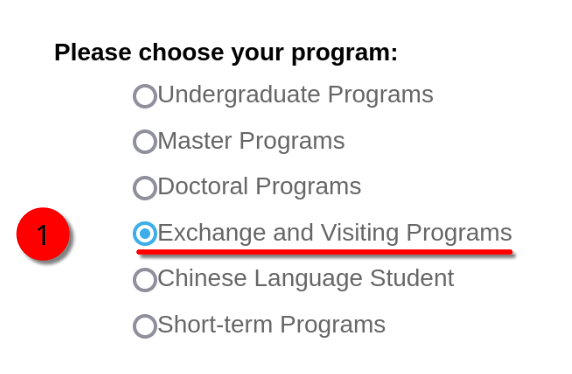
\includegraphics[width=\textwidth]{russia/imgs/app_1}
    \end{subfigure}
    \hfill
    \begin{subfigure}[c]{0.49\textwidth}
        \centering
        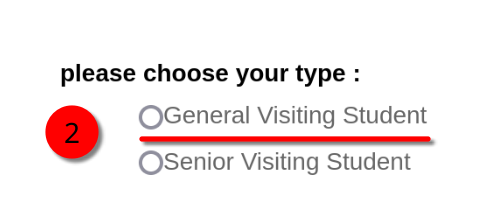
\includegraphics[width=\textwidth]{russia/imgs/app_2}
    \end{subfigure}
    \caption{Positive samples of Canny Edge Algorithm}
    \label{fig:ru_student_type}
\end{figure}



After, you should specify the Department and Major.
For Department \textcircled{1} and Major \textcircled{2} choose
\textbf{``Computer Science and Technology``}.
Don't forget to specify the English language \textcircled{3}!
Start the search \textcircled{4} and choose appropriate study plan \textcircled{5}.
Additionally, pay attention to application period!
Maybe the application period not started yet.
Fig~\ref{fig:ru_study_plan}


\begin{figure}[htpb]
    \centering
    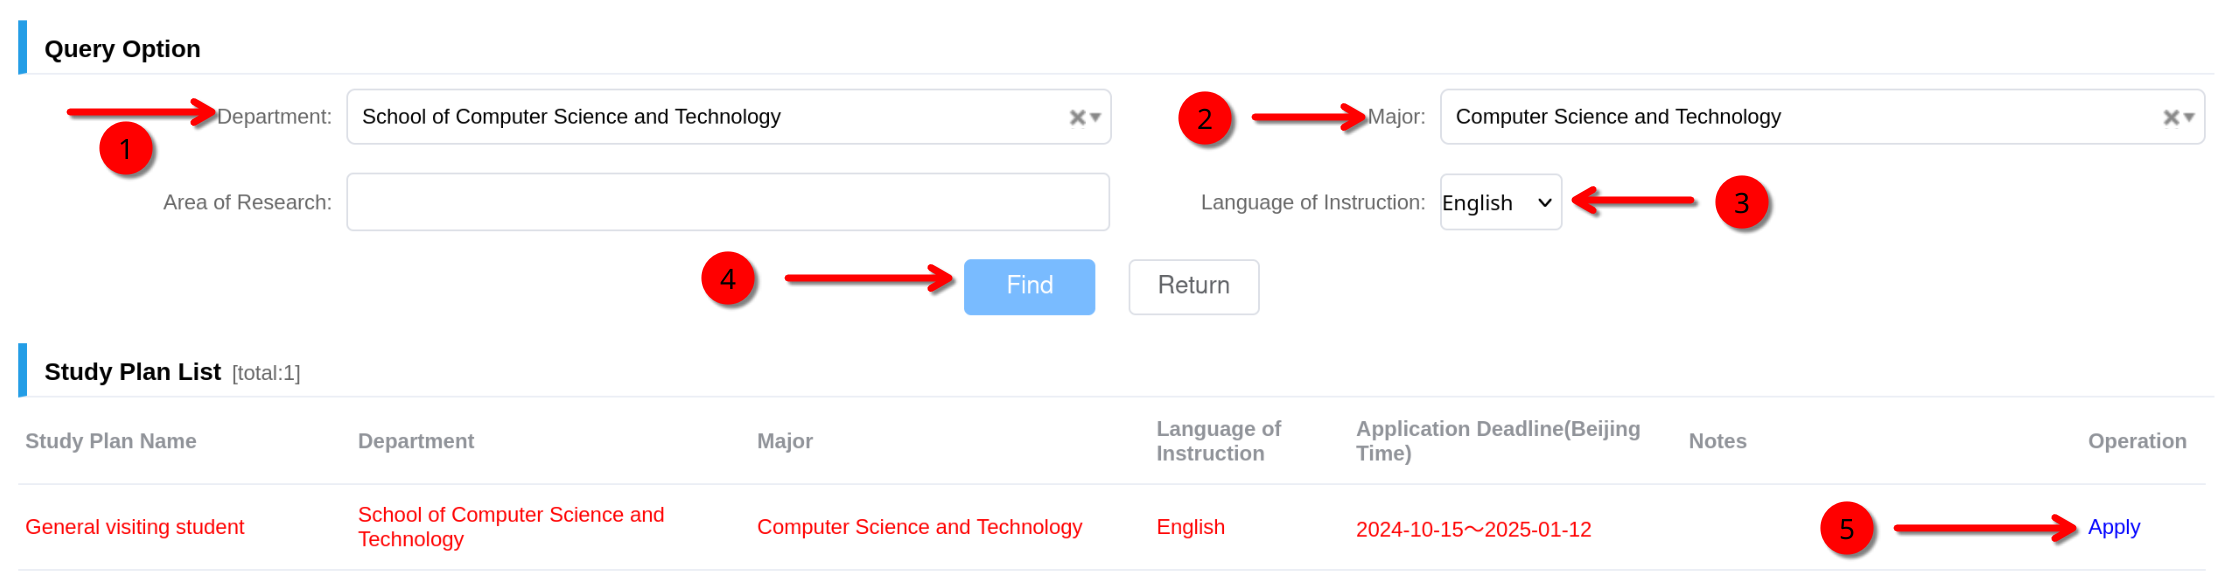
\includegraphics[width=\textwidth]{russia/imgs/app_3_study_plan}
    \caption{\centering Study Plans}
    \label{fig:ru_study_plan}
\end{figure}


\section{Personal Information}\label{sec:ru_personal_info}

This section not that hard, but some points should be clarified!
Fig~\ref{fig:ru_pers_info}

\begin{enumerate}
    \item Fill the name and surname according to international passport.
        If you still don't have it, you can check spelling
        \href{https://www.gosuslugi.ru/help/faq/foreign_passport/100359}{HERE}.

    \item \textbf{Highest Level of Education}: Bachelor

    \item \textbf{Final Education Institution}: Innopolis University

    \item \textbf{Occupation}: Student

    \item \textbf{Chinese Name}.
        If you don't have Chinese name yet, leave field blank.
        The Chinese coordinator will give you Chinese names that match the real ones. \\
        \textbf{For example}: Timofei - MoFei, Artur - AnTeng (it may sound not that similar)

    \item \textbf{Employer or Institution Affiliated}: Innopolis University
\end{enumerate}


\begin{figure}[H]
    \centering
    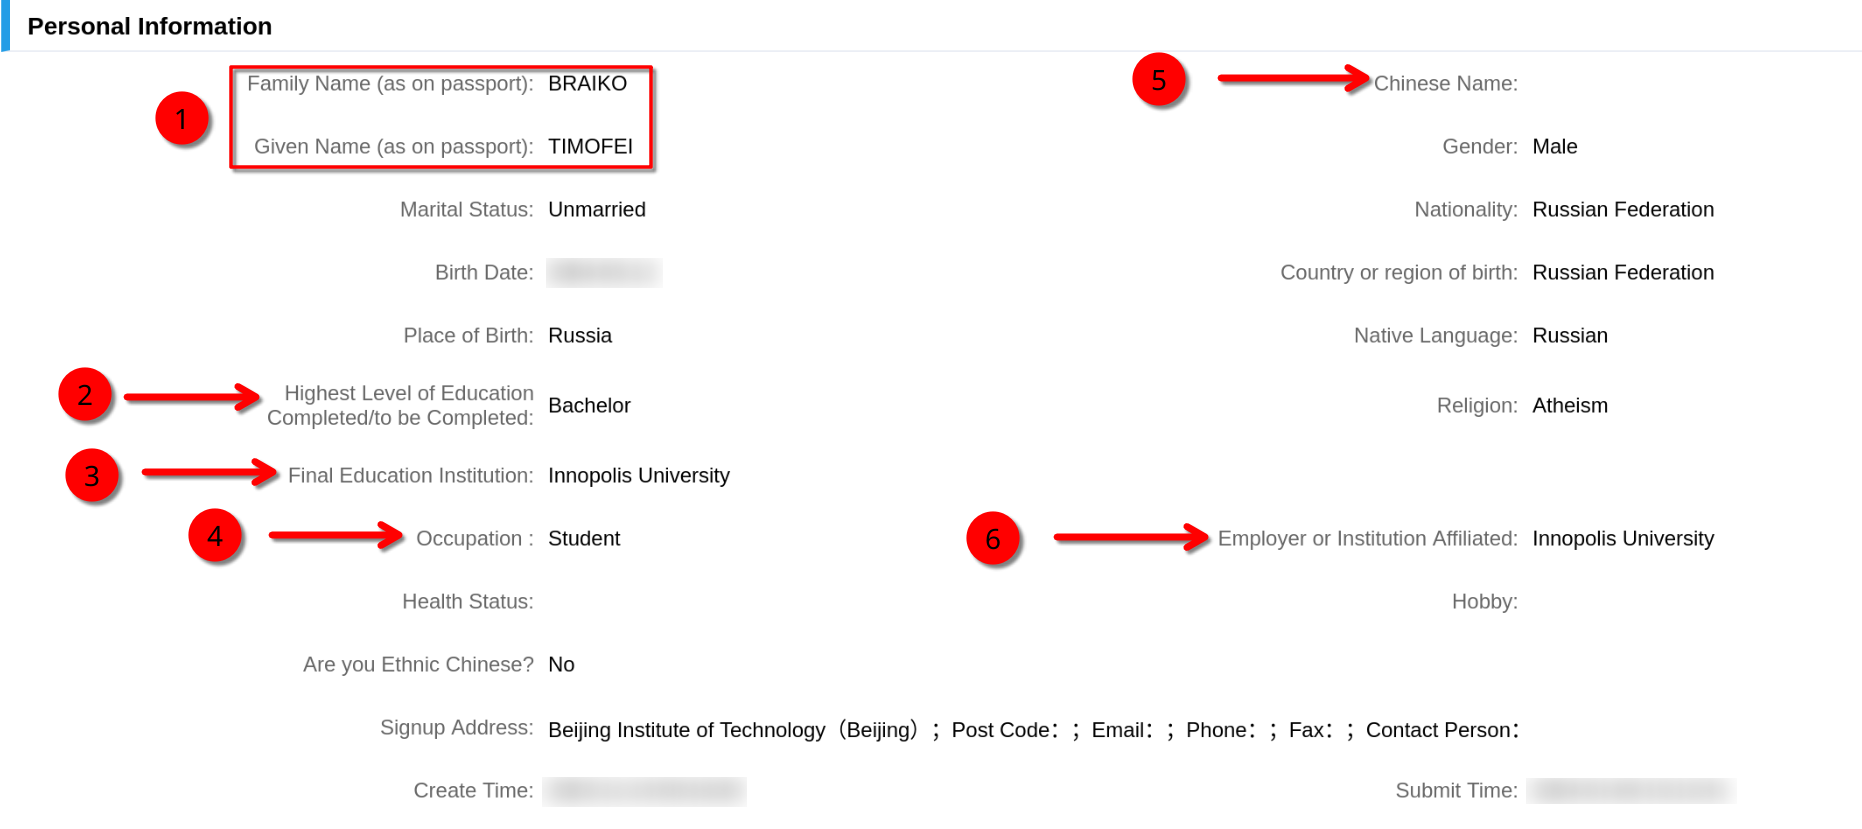
\includegraphics[width=\textwidth]{russia/imgs/app_4_personal_info}
    \caption{\centering Personal Information}
    \label{fig:ru_pers_info}
\end{figure}


\section{Passport}

In this section, you fill in your international passport details.

Regarding field \textbf{Location of Visa Office}.
At the end of 2024, a Chinese visa can be obtained in the following places:

\begin{itemize}
    \item \textbf{Embassy in Russia Federation} - Moscow
    \item \textbf{Consulate in St.Petersburg}
    \item \textbf{Consulate in Yekaterinburg}
    \item \textbf{Consulate in Khabarovsk}
    \item \textbf{Consulate in Vladivostok}
\end{itemize}


\begin{tcolorbox}[colback=yellow!10, colframe=yellow!80!black, title=Note]
    At the time of writing, a visa cannot be obtained in Kazan.
\end{tcolorbox}


\section{Language Proficiency}
Enter the exam results.
Please note that if you have passed the IELTS or TOEFL yourself,
they are valid for only two years.
If you passed inner-university exam choose IELTS, as it's based on IELTS exam.
Issue date is printed on certificate Fig~\ref{fig:ru_lang_prof}.


\begin{figure}[H]
    \centering
    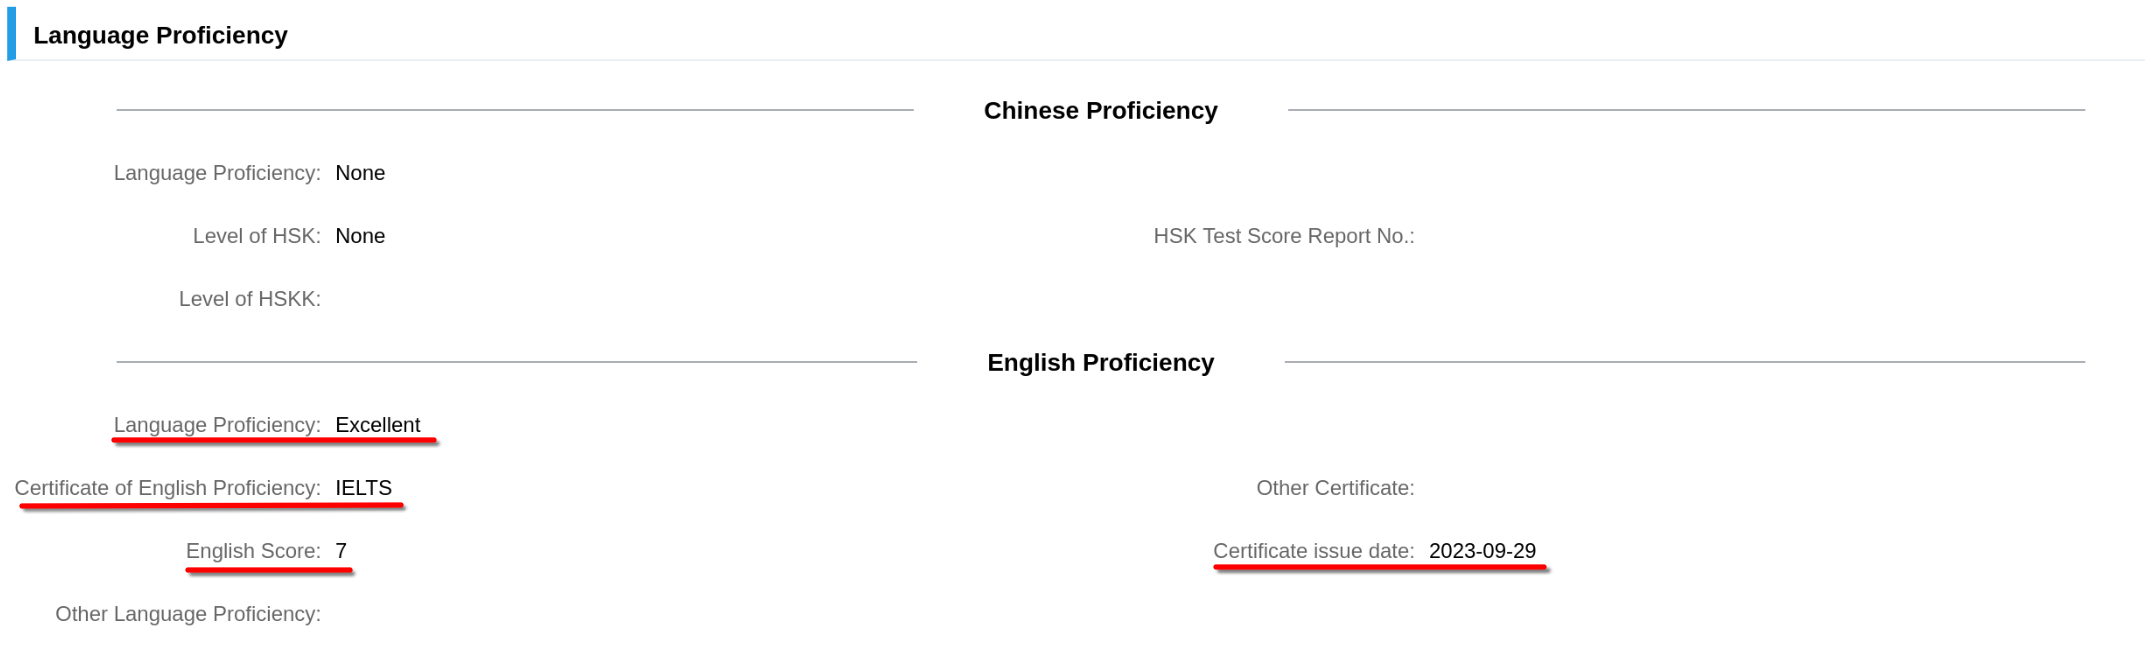
\includegraphics[width=\textwidth]{russia/imgs/app_5_language}
    \caption{\centering Language Proficiency}
    \label{fig:ru_lang_prof}
\end{figure}



\section{Recommender}
Specify the head of the department here.
For this moment, he is Petr Zhdanov Fig~\ref{fig:ru_recommender}.

\begin{itemize}
    \item \textbf{Source:} Others - Head of the International Relation Office
    \item \textbf{Name:} Petr Zhdanov
    \item \textbf{Organization:} Autonomous noncommercial organization of higher education ``Innopolis University``.
    \item \textbf{Phone Number:} +7 843 203 92 53
    \item \textbf{Relationship with applicant:} Head of the International Relation Office
    \item \textbf{Email:} pe.zhdanov@innopolis.ru
\end{itemize}


\begin{figure}[H]
    \centering
    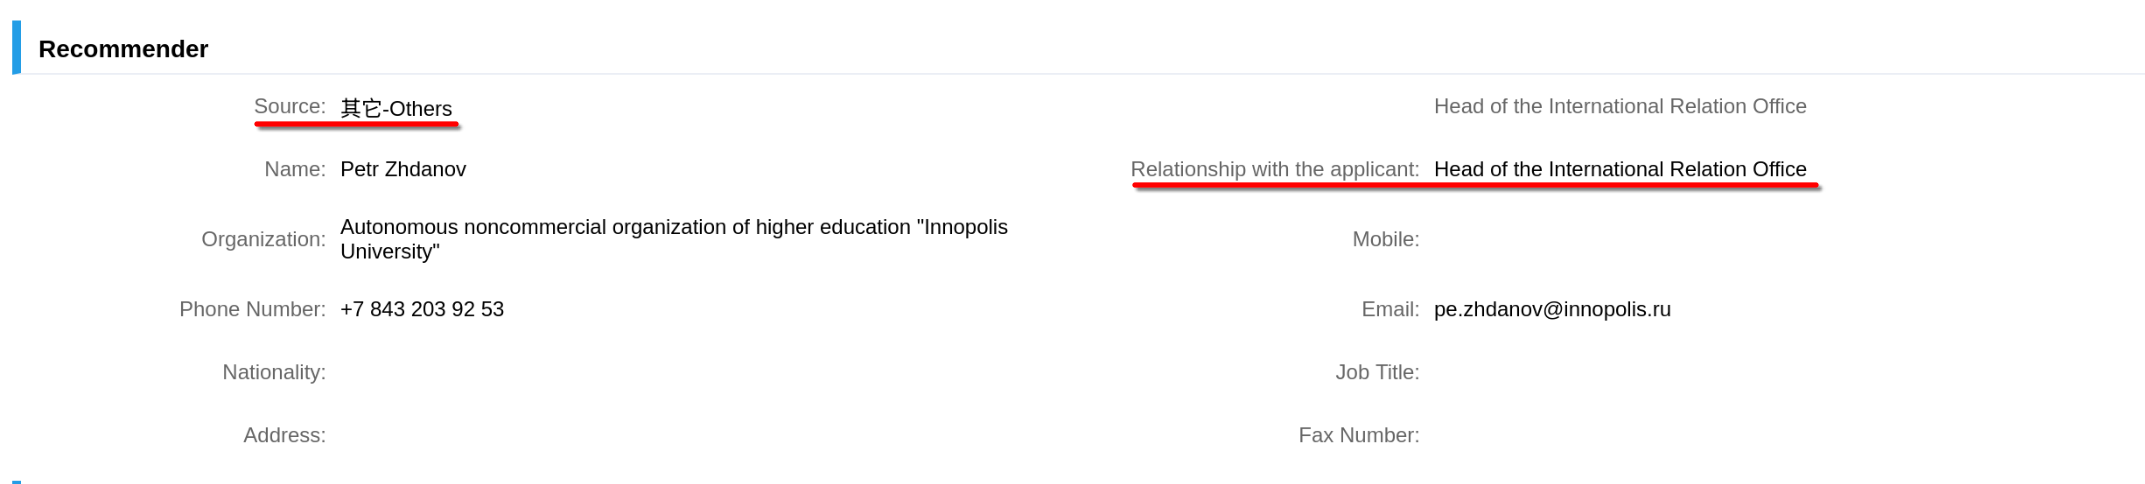
\includegraphics[width=\textwidth]{russia/imgs/app_6_recommender}
    \caption{\centering Recommender}
    \label{fig:ru_recommender}
\end{figure}


\section{}




	\part[China]{China}\label{part:cn}
	%! Author = a
%! Date = 1/27/25


\chapter{Introduction}\label{ch:ru_introduction}
Hello, World!


\chapter{BIT Application}\label{ch:ru_application}

After you were qualified for the exchange program,
you need to sign up for an exchange program on
\href{https://apply.isc.bit.edu.cn/apply/}{the BIT website}.
Go to the website \url{https://apply.isc.bit.edu.cn/apply/},
register and click on \textit{Start Application}.

\begin{tcolorbox}[colback=yellow!10, colframe=yellow!80!black, title=Note]
    Google is banned in China.
    We recommend to use Yandex or University email
    for registration and other purposes.
\end{tcolorbox}


\section{Study Plan}\label{sec:study_plan}

Firstly, choose \textcircled{1} \textbf{``Exchange and Visiting Programs``},
as you apply for the exchange program.
On the next page if you are a bachelor student (undergraduate),
choose \textcircled{2} \textbf{``General Visiting Student``}.
For masters, choose \textbf{``Senior Visiting Student``}
Fig~\ref{fig:ru_student_type}.


\begin{figure}[htbp]
    \centering
    \begin{subfigure}[c]{0.49\textwidth}
        \centering
        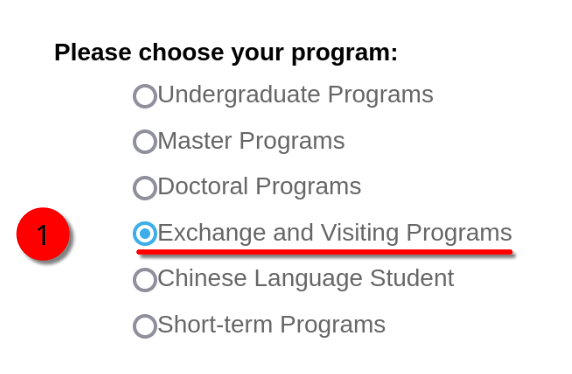
\includegraphics[width=\textwidth]{russia/imgs/app_1}
    \end{subfigure}
    \hfill
    \begin{subfigure}[c]{0.49\textwidth}
        \centering
        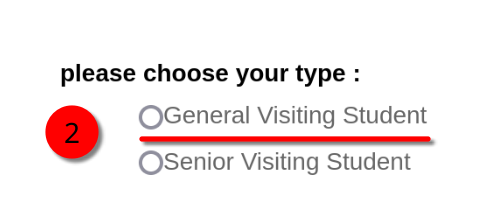
\includegraphics[width=\textwidth]{russia/imgs/app_2}
    \end{subfigure}
    \caption{Positive samples of Canny Edge Algorithm}
    \label{fig:ru_student_type}
\end{figure}



After, you should specify the Department and Major.
For Department \textcircled{1} and Major \textcircled{2} choose
\textbf{``Computer Science and Technology``}.
Don't forget to specify the English language \textcircled{3}!
Start the search \textcircled{4} and choose appropriate study plan \textcircled{5}.
Additionally, pay attention to application period!
Maybe the application period not started yet.
Fig~\ref{fig:ru_study_plan}


\begin{figure}[htpb]
    \centering
    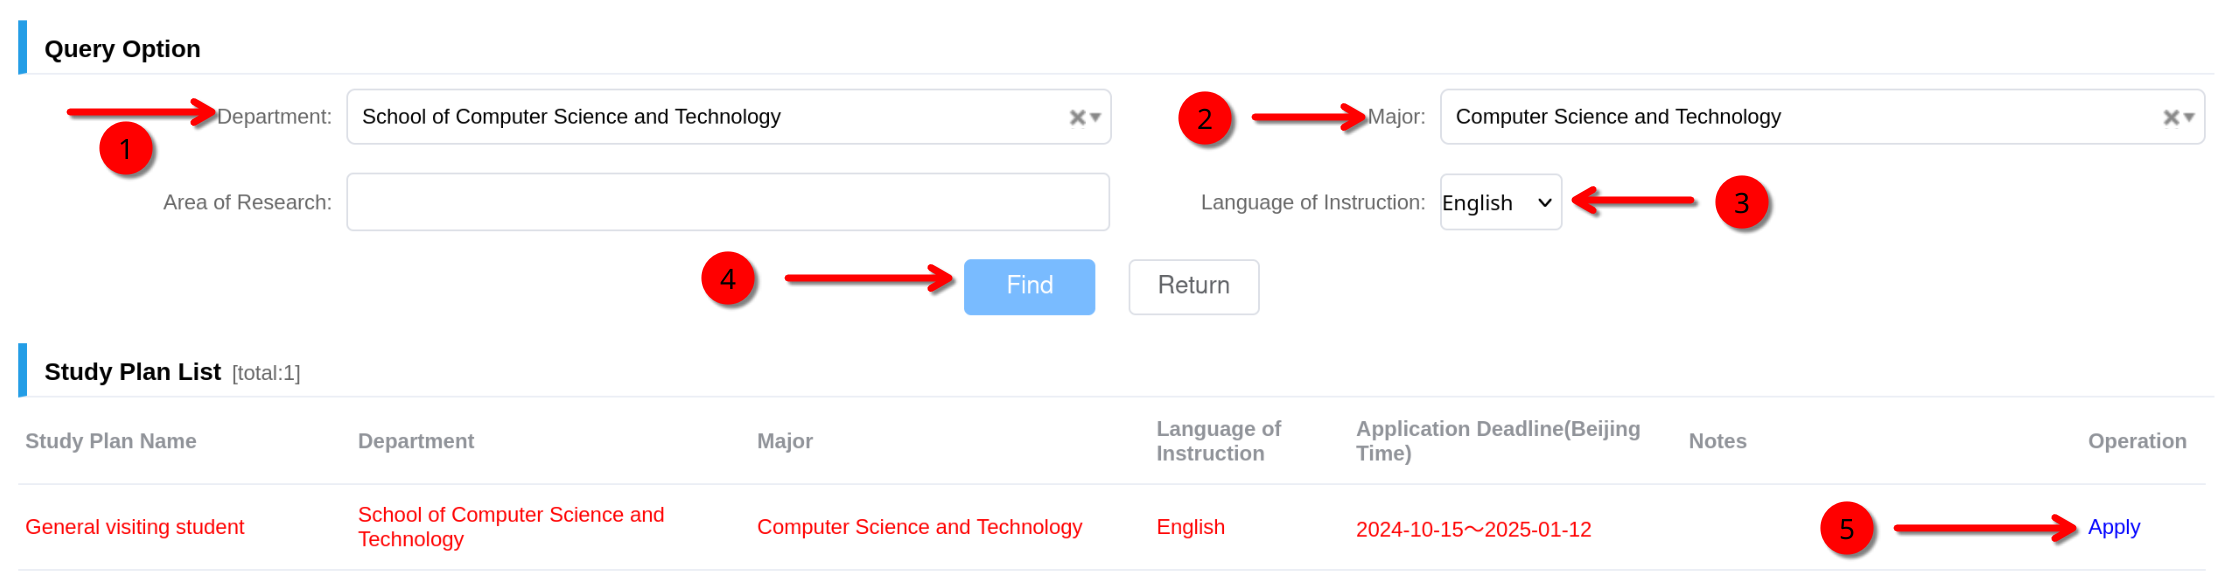
\includegraphics[width=\textwidth]{russia/imgs/app_3_study_plan}
    \caption{\centering Study Plans}
    \label{fig:ru_study_plan}
\end{figure}


\section{Personal Information}\label{sec:ru_personal_info}

This section not that hard, but some points should be clarified!
Fig~\ref{fig:ru_pers_info}

\begin{enumerate}
    \item Fill the name and surname according to international passport.
        If you still don't have it, you can check spelling
        \href{https://www.gosuslugi.ru/help/faq/foreign_passport/100359}{HERE}.

    \item \textbf{Highest Level of Education}: Bachelor

    \item \textbf{Final Education Institution}: Innopolis University

    \item \textbf{Occupation}: Student

    \item \textbf{Chinese Name}.
        If you don't have Chinese name yet, leave field blank.
        The Chinese coordinator will give you Chinese names that match the real ones. \\
        \textbf{For example}: Timofei - MoFei, Artur - AnTeng (it may sound not that similar)

    \item \textbf{Employer or Institution Affiliated}: Innopolis University
\end{enumerate}


\begin{figure}[H]
    \centering
    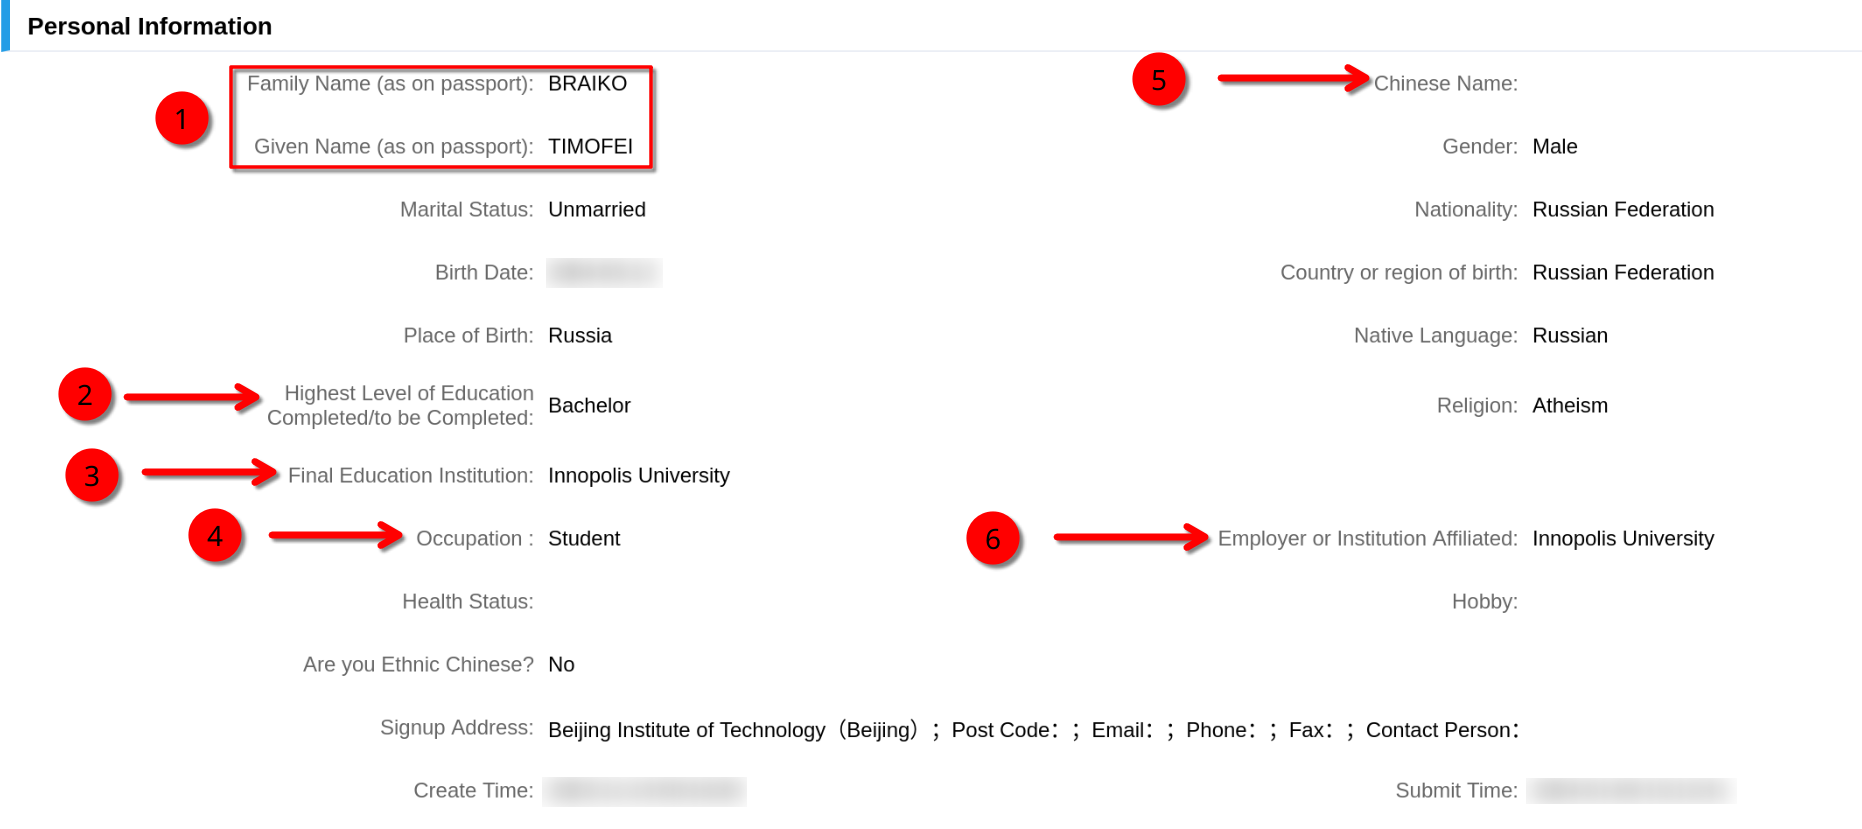
\includegraphics[width=\textwidth]{russia/imgs/app_4_personal_info}
    \caption{\centering Personal Information}
    \label{fig:ru_pers_info}
\end{figure}


\section{Passport}

In this section, you fill in your international passport details.

Regarding field \textbf{Location of Visa Office}.
At the end of 2024, a Chinese visa can be obtained in the following places:

\begin{itemize}
    \item \textbf{Embassy in Russia Federation} - Moscow
    \item \textbf{Consulate in St.Petersburg}
    \item \textbf{Consulate in Yekaterinburg}
    \item \textbf{Consulate in Khabarovsk}
    \item \textbf{Consulate in Vladivostok}
\end{itemize}


\begin{tcolorbox}[colback=yellow!10, colframe=yellow!80!black, title=Note]
    At the time of writing, a visa cannot be obtained in Kazan.
\end{tcolorbox}


\section{Language Proficiency}
Enter the exam results.
Please note that if you have passed the IELTS or TOEFL yourself,
they are valid for only two years.
If you passed inner-university exam choose IELTS, as it's based on IELTS exam.
Issue date is printed on certificate Fig~\ref{fig:ru_lang_prof}.


\begin{figure}[H]
    \centering
    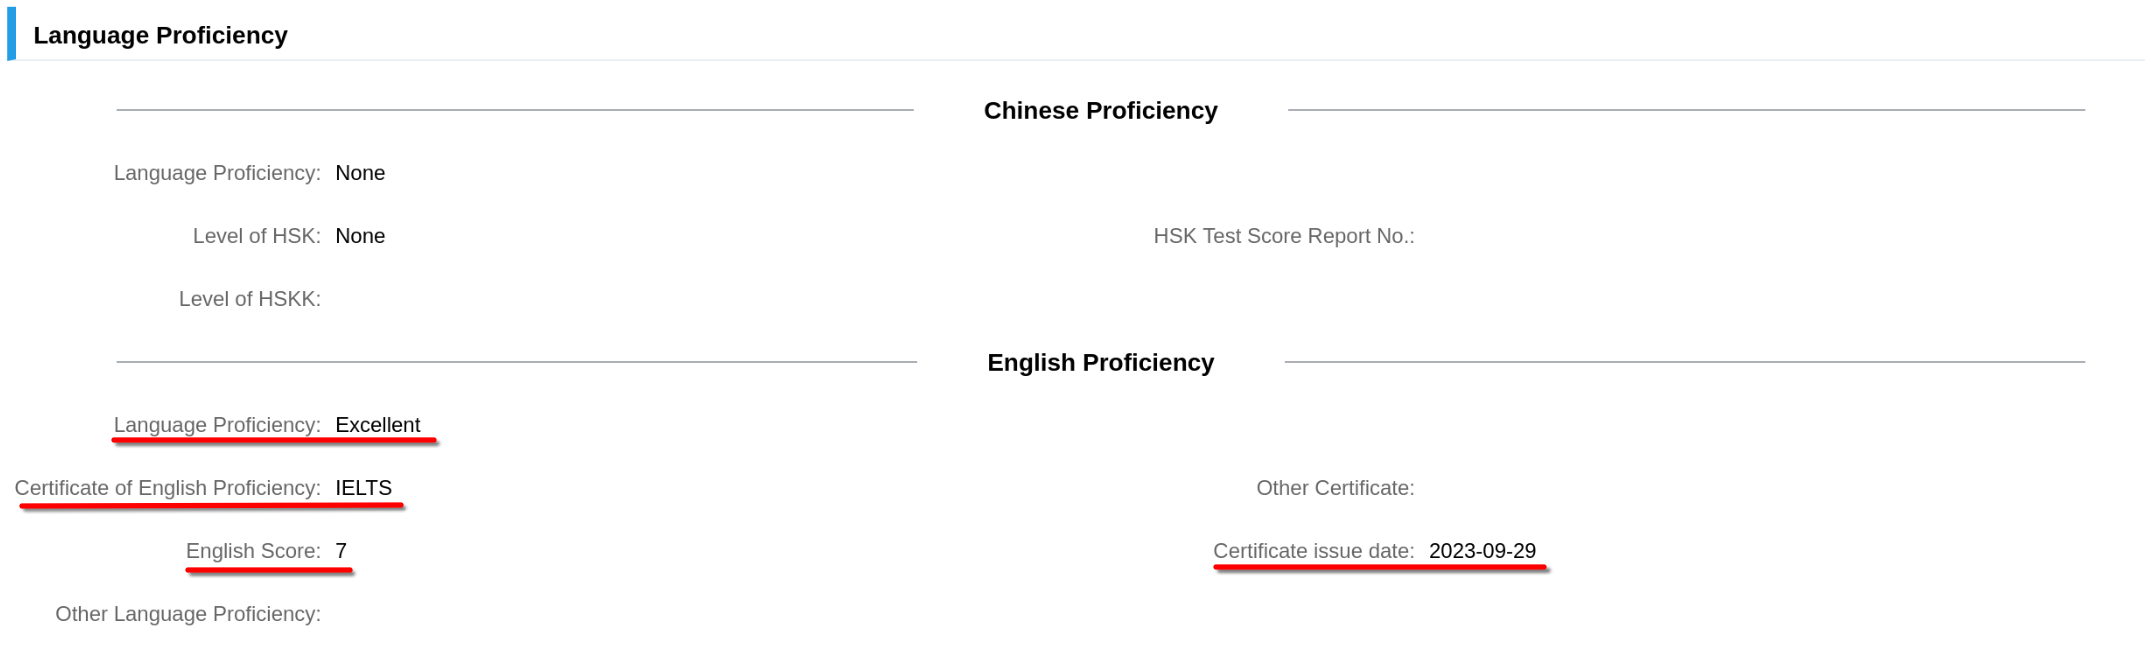
\includegraphics[width=\textwidth]{russia/imgs/app_5_language}
    \caption{\centering Language Proficiency}
    \label{fig:ru_lang_prof}
\end{figure}



\section{Recommender}
Specify the head of the department here.
For this moment, he is Petr Zhdanov Fig~\ref{fig:ru_recommender}.

\begin{itemize}
    \item \textbf{Source:} Others - Head of the International Relation Office
    \item \textbf{Name:} Petr Zhdanov
    \item \textbf{Organization:} Autonomous noncommercial organization of higher education ``Innopolis University``.
    \item \textbf{Phone Number:} +7 843 203 92 53
    \item \textbf{Relationship with applicant:} Head of the International Relation Office
    \item \textbf{Email:} pe.zhdanov@innopolis.ru
\end{itemize}


\begin{figure}[H]
    \centering
    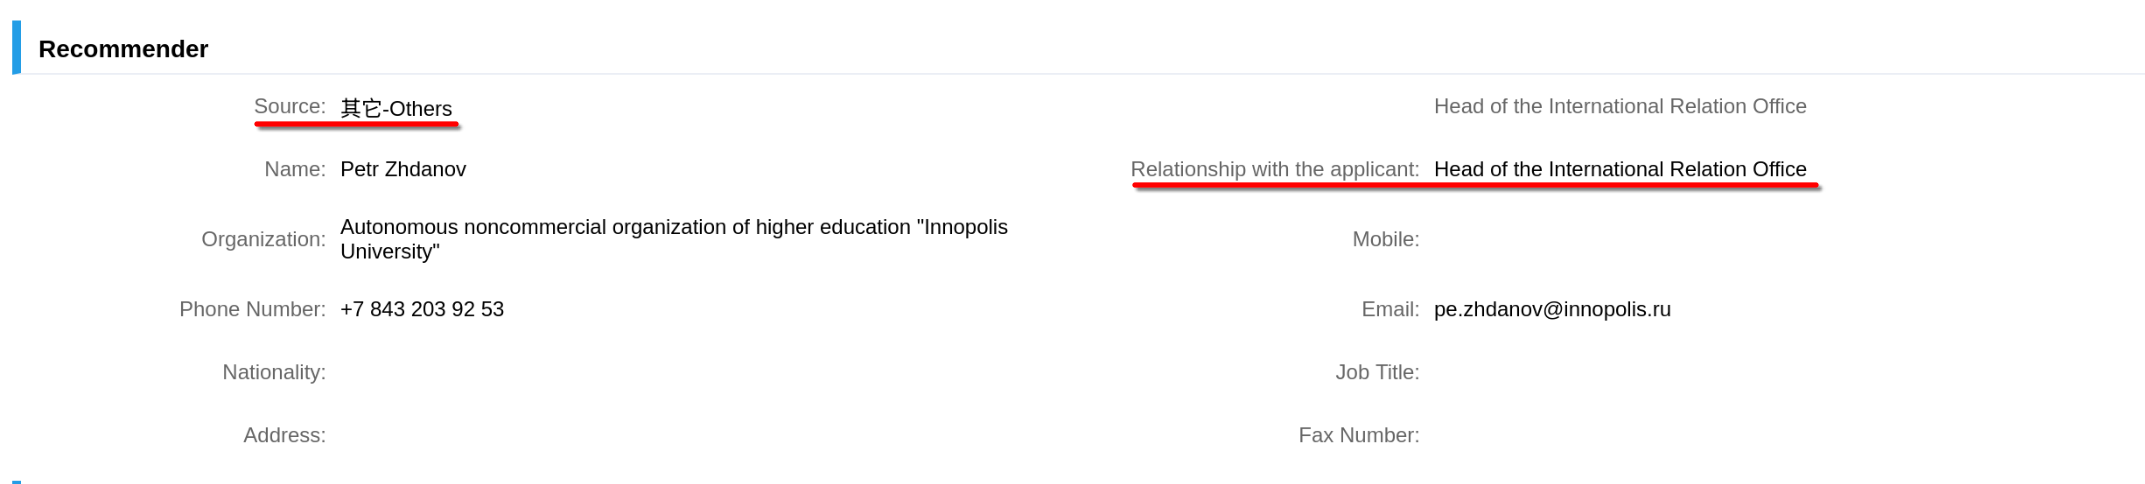
\includegraphics[width=\textwidth]{russia/imgs/app_6_recommender}
    \caption{\centering Recommender}
    \label{fig:ru_recommender}
\end{figure}


\section{}




	\bibliography{main}
	\bibliographystyle{plain}

\end{document}
